\documentclass[twocolumn,twoside,a4paper, 10pt]{article}
\usepackage[utf8]{inputenc}
\usepackage[T1]{fontenc}
\usepackage[spanish]{babel}
\usepackage{balance}
\usepackage{jenuia4}
\usepackage{url}
\usepackage{graphicx}

\usepackage{hyperref}

\title{El impacto de la IA en la enseñanza de la programación}

%\author{\normalsize 
%\begin{tabular}{@{\extracolsep{3mm}}cc}
%{\large Joe Miró Julià }                  & {\large Mercedes Marqués}\\
%Departament de Matemàtiques i Informàtica & Departamento de Ing. y Ccia. de los Comput.\\
%Universitat de les Illes Balears          & Universitat Jaume I\\
%07122 Palma de Mallorca                   & Castellón\\
%\url{joe.miro@uib.es}                     & \url{merche.marques@uji.es}
%\end{tabular}
%}

\author{ \small
\begin{tabular}{@{\extracolsep{3mm}}c}
\large Francisco de Sande \\
Departamento de Ingeniería Informática y de Sistemas \\
Universidad de La Laguna \\
38200 La Laguna. S/C de Tenerife \\
fsande@ull.es
\end{tabular}
}

\date{}

%%%  Referencias
% https://aihub.csic.es/inteligencia-artificial-en-educacion-golem-creativo-o-destructor/

\begin{document}
\maketitle
\thispagestyle{empty}

\begin{abstract}
\noindent Abstract
\end{abstract}

\section*{Abstract}
\noindent Abstract Pedirle que los ids del código sean significativos.

\section*{Palabras clave}
\noindent Programación IA ChatGPT GitHub Copilot Enseñanza Informática Evaluación

\section{Pruebas}
Jutge \cite{URL::Jutge, Petit:Jutge:2018}

Comenzar a hablar de lo que hacems en IB para evaluar las prácticas de programación.
Descripción de la asignatura, temario, etc.

chatGPT \cite{Zhang:2020:chatgpt, Castelvecchi:2022:ACaA}

AlphaCode \cite{Li:2022:CCG}


En junio de 2021, GitHub lanzó Copilot \cite{Friedman:2021:IGC}, un "programador de pares de IA" que genera 
código en diversos lenguajes a partir de cierto contexto como comentarios, nombres de funciones y código adyacente. 
Copilot se basa en un modelo que se entrena con código abierto \cite{Chen:2021:ELL}, incluido "código público... 
con patrones de codificación inseguros, lo que da lugar a la posibilidad de sintetizar código que contenga 
estos patrones indeseables".

\section{Introducción}
\textit{Informática Básica} (IB, de ahora en adelante) es una asignatura de 6 créditos que se imparte en el primer cuatrimestre 
del primer curso del Grado en Ingeniería Informática en la Escuela Superior de Ingeniería y Tecnología de la
Universidad de La Laguna.

Se trata de la primera asignatura (y única en ese primer cuatrimestre) de perfil eminentemente informático que
cursa el alumnado del título de Grado.
El número de estudiantes que habitualmente cursa la asignatura está en torno a los 250. 
Los contenidos de la asignatura pueden consultarse en la Guía Docente \cite{ULL:2022:GD} de la misma.
Al margen de un par de temas dedicados a una introducción a las Bases de Datos, Redes y Sistemas Operativos,
el grueso de los contenidos (en torno a 12 de las 15 semanas del cuatrimestre) se dedican a introducir al
alumnado en la materia de Programación, siendo C++ el lenguaje vehicular elegido para estudiar la materia.
Se trata de una asignatura con una importante proporción de contenidos prácticos en la que cada estudiante
recibe 4 horas presenciales de clase a la semana distribuídas del siguiente modo:
\begin{itemize}
  \item 2 horas dedicadas al estudio de contenidos teóricos
  \item 1 hora dedicada a la resolución de Problemas
  \item 1 horas de Prácticas
\end{itemize}
La Guía docente establece que por cada hora de trabajo presencial, cada estudiante debería dedicar en 
promedio 1,5 horas de trabajo autónomo, de modo que se espera unas 6 horas de trabajo autónomo semanal por 
parte de cada estudiante. 
Se describe a continuación el tipo de actividades que se desarrolla en cada una de este tipo de sesiones.

Las sesiones destinadas a contenidos teóricos se imparten con el formato de clase expositiva y se dedican, 
con el uso de transparencias que el alumnado tiene disponibles a través del aula virtual, al estudio de los 
contenidos de la asignatura. 
Junto a las transparencias, el alumnado dispone de una serie de pequeños programas que sirven de ilustración a
los contenidos que se estudian en clase. 
Se recomienda al alumnado estudiar esos programas para afianzar sus conocimientos de cada tema.

En las sesiones de problemas el profesorado utiliza un terminal cuya pantalla se proyecta a toda la clase para
resolver algunos problemas seleccionados, resolviendo al mismo tiempo las dudas que puedan surgir en esa
resolución. 

Cada semana al alumnado se le propone la realización de una práctica, consistente en un cierto número (cinco
es el número frecuente) de programas en C++ relacionados con algún tema estudiado.
Esos programas tienen el propósito de servir de "entrenamiento" para el alumnado para afianzar conocimientos y
el alumnado dispone de una semana para realizar esos ejercicios.
La sesión semanal de prácticas se destina a la evaluación de esos conocimientos a través de la realización de
ejercicios de programación de complejidad similar a los que han sido propuestos con antelación.
En algunos casos los ejercicios de evaluación son simples modificaciones de los que se han propuesto para
realizar con antelación.

% Porcentajes de la evaluación
% 10 minutos para cuestionarios

\section{Motivación}
La evaluación de las prácticas de programación del alumnado de IB ha sido siempre una dificultad en el
desempeño docente de esta asignatura. 
La dificultad es compartida por muchas otras asignaturas de la titulación que tienen una significativa
componente práctica en sus contenidos, de modo que casi todas las cuestiones que en este trabajo queremos
plantear son comunes a muchas asignaturas e incluso a otras titulaciones.

Esta dificultad es polifacética y no se puede analizar desde un único punto de vista.

Por una parte, la programación es una actividad transversal a cualquier especialización de la informática y su
importancia es ubicua en esta titulación.
Los conceptos inherentes a la programación de ordenadores son comunes, con pequeñas variaciones, a los
diferentes lenguajes de programación.
En IB hemos decidido optar por C++ como lenguaje vehicular para aprender programación, pero este lenguaje bien
pudiera haber sido Python, Java o JavaScript.
Forzando un poco las similitudes podríamos decir que la programación se asemeja a las habilidades para
conducir un automóvil: cualquier persona con permiso para conducir puede decir que conduce correctamente, pero
decir que se es una buena conductora requiere muchas horas de práctica y exposición a situaciones anormales.
Del mismo modo cualquier informático dirá que sabe programar pero sus habilidades en esta materia dependerán
muy directamente del número de horas de entrenamiento que se hayan dedicado a la misma.

Siguiendo esta idea, recomendamos encarecidamente al alumnado de IB que realicen cuantos ejercicios prácticos
sean capaces para, de forma progresiva, ir incrementando sus capacidades como programadores.
%%%%%%%%%%%%%%%%%%%% Table %%%%%%%%%%%%%%%%%%%%%%%%%%%%%%%%%%%
%\begin{table*}
%	\begin{center}
%	\begin{tabular}{p{5.2cm}p{4.5cm}cc}
%		\textbf{Título} & \textbf{Autores} & \textbf{Edición} & 
%		\textbf{Citas (Heterocitas)}\\\hline
%		Niveles de Competencia de los Objetivos Formativos en las 
%		Ingenierías & Miguel Valero-Garcia y Juan José Navarro & 2001 
%		& 21 (18) \\\hline
%		Formulación de los Objetivos de una Asignatura en Tres Niveles
%		Jerárquicos & Juan José Navarro, Miguel Valero-Garcia, Fermín
%		Sánchez Carracedo y Jordi Tubella & 2000 & 18 (8) \\\hline
%		¿Cómo serán las asignaturas del EEES? & Fermín Sánchez
%		Carracedo & 2005 & 10 (6) \\\hline
%		Evaluación continuada a un coste razonable & Miguel
%		Valero-Garcia, Luís M. Díaz de Cerio & 2002 & 9 (9) \\\hline
%		Hacia la Evaluación Continua Automática de Prácticas de
%		Programación & Juan Carlos Rodríguez del Pino, Margarita Díaz
%		Roca, Zenón J. Hernández Figueroa y José Daniel González
%		Domínguez & 2007 & 8 (7) 
%	\end{tabular}
%	\end{center}
%	\caption{\label{tab:mascit}Artículos más citados en las Jenui.}
%\end{table*}
%%%%%%%%%%%%%%%%%%%%%%%%%%%%%%%%%%%%%%%%%%%%%%%%%%%%%%%%%%%%%%

\section{Títulos y apartados}

El título de la obra debe estar a 18~puntos, en negrita y centrado.

\section{Extensión}

El número máximo de páginas que se pueden utilizar es de 8~páginas para las ponencias 
y para las descripciones de los recursos docentes, y de 4~páginas para los pósteres 
(en ediciones anteriores, los pósteres estaban limitados a 2~páginas). 
Es imprescindible que los autores utilicen el formato y se ajusten al espacio ya 
desde la primera versión que se someta al proceso de revisión. Lo contrario implicaría 
el rechazo de la contribución.

\section{Listas}

A menudo encontramos listas en las ponencias de las Jenui. 
Cada elemento de la lista va precedido de un símbolo o un número y 
el texto de la lista usa de una línea más estrecha que la del texto. 
Las normas de edición de las listas se muestran a continuación.

\begin{itemize}
	\item Los símbolos que preceden a cada elemento de la lista son 
	números en el caso de listas enumeradas o \emph{balas} 
	($\bullet$) si la lista no está enumerada.
	
	\item La distancia del margen izquierdo del texto de la lista al
	margen izquierdo de la columna (el texto normal) es de 7~mm.  El
	margen derecho de la lista es el mismo que el margen derecho de la
	columna. Es decir, que la anchura de texto de la lista es de 69,5~mm.
	
	\item La distancia del extremo derecho del símbolo al texto de la 
	lista es de 1,5 mm. Los números crecen hacia la izquierda: si hay 
	un número de dos dígitos, el segundo dígito acaba a 1,5 mm del 
	texto de la lista.
	
	\item La distancia adicional del primer elemento de la lista al texto que 
	le precede es aproximadamente de 1,4~mm. Esta también es la distancia adicional del último 
	elemento de la lista al texto que le sucede.
	
	\item Está prohibido tener más de un nivel de 
	listas. Es decir, no se pueden tener listas dentro de listas.
\end{itemize}

\section{Figuras y cuadros}

Las figuras y los cuadros pueden ir dentro de una columna (anchura 
máxima 76,5~mm) o dentro del cuerpo (anchura máxima 160~mm). En ambos 
casos la figura o el cuadro van centrados dentro de la columna o el 
cuerpo. Ambas van numeradas y tienen numeraciones independientes. El 
pie de figura o cuadro empieza con \emph{Figura n:} o \emph{Cuadro 
n:} y usa texto normal a 10~puntos. El pie  va separado 
aproximadamente por la altura de una línea (4~mm) a la figura o 
cuadro y está centrado. La distancia entre el pie y el texto es de 
aproximadamente dos líneas (9~mm).

%%%%%%%%%%%%%%%%%%%% Fig. %%%%%%%%%%%%%%%%%%%%%%%%%%%%%%%%%%%
%\begin{figure}[htbp]
%\centerline{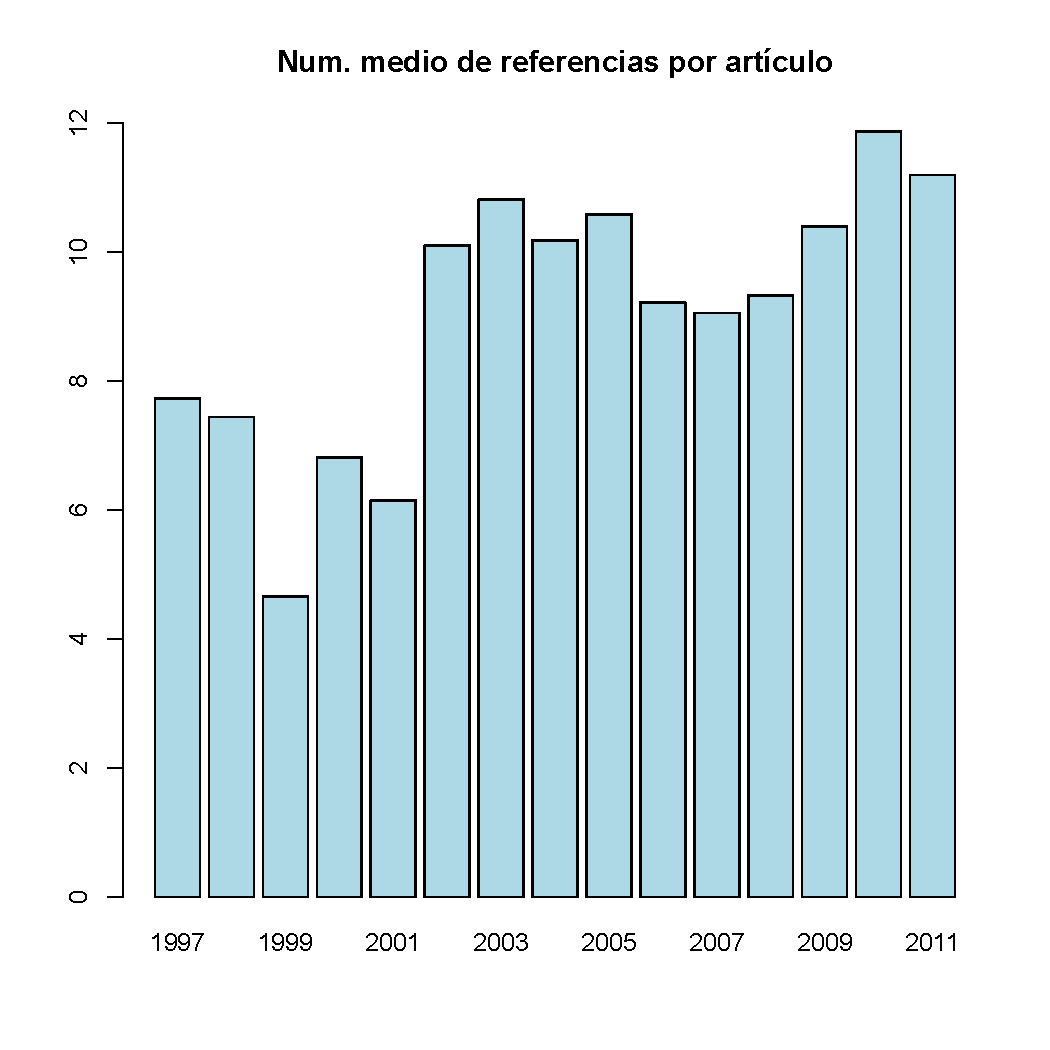
\includegraphics[width=\linewidth]{mediaref}}
%\caption{\label{fig:medias} Número medio de referencias por artículo en las 15 ediciones de las Jenui} 
%\label{fig:} 
%\end{figure}
%%%%%%%%%%%%%%%%%%%%%%%%%%%%%%%%%%%%%%%%%%%%%%%%%%%%%%%%%%%%%%

%%%%%%%%%%%%%%%%%%%% Fig. %%%%%%%%%%%%%%%%%%%%%%%%%%%%%%%%%%%
%\begin{figure*}
%	\begin{center}
%	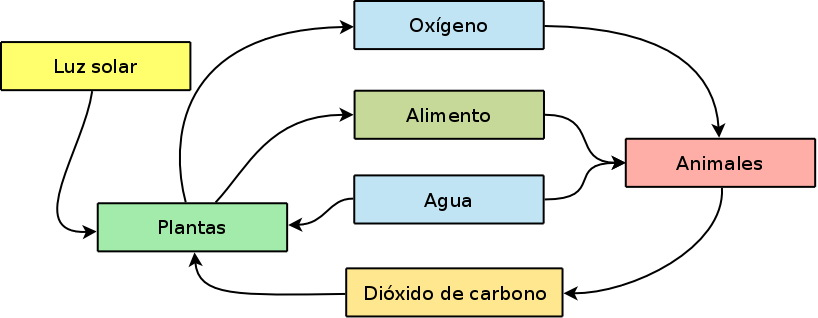
\includegraphics[width = 0.8\linewidth]{diagrLargo.jpg}
%	\end{center}
%	\caption{Diagrama en ancho de dos columnas.}
%\end{figure*}
%%%%%%%%%%%%%%%%%%%%%%%%%%%%%%%%%%%%%%%%%%%%%%%%%%%%%%%%%%%%%%

\section{Bibliografía}
En el texto se utiliza el número de la referencia, también entre 
corchetes. Hay tres cuestiones a tener en cuenta: (a) El número de 
referencia no puede empezar una línea, hay que poner un ``blanco 
duro'' entre el número de referencia y el texto que lo precede; (b) 
Si hay varias referencias juntas debe usarse un único par de 
corchetes: debe ser ``[2, 7, 14]'' y no ``[2][7][14]''; (c) Si hay 
varias referencias, deben ir en orden numérico ascendente: debe ser  
``[2, 7, 14]'' y no ``[14, 2, 7]''.

El formato de la bibliografía casi merece un artículo propio. 
Recomendamos que las referencias bibliográficas se incluyan en un fichero 
independiente así como el uso del estilo \textit{jenui}. Éste es una adaptación al castellano 
del clásico estilo \textit{plain}.
Si se usa un programa bibliográfico como BibTeX, o EndNote no es necesario 
preocuparse de mucho. En cambio, si se crea la bibliografía a mano 
recomendamos que se mire este artículo o un libro adecuado como 
referencia y que se sigan las siguientes normas:
%
\begin{itemize}
	\item Se debe ser consistente.  Por ejemplo si en una entrada se
	pone ``Actas de las XVII Jornadas de Enseñanza Universitaria de la
	Informática'' en otra no puede ponerse ``Jenui 2012'' y en otra
	``Actas del Jenui'98''.  Si en una entrada el título de un libro
	va en cursiva, en otra entrada no puede ir en letra normal.  No
	importa tanto cómo se escriba sino que siempre se escriba igual.
	
	\item Todo debe ir en español.  Si se importa la bibliografía de
	otra fuente (o se usa BibTeX) es posible que se importen palabras
	en inglés (``J. García \emph{and} P. Quintero, \emph{editors}'').
	Debe cambiarse al español\footnote{Usuarios de BibTeX: editad el
	archivo .bbl justo antes de la última compilación.}. Si se usa el estilo
	\textit{jenui} no es necesario hacer cambios en el nombre de los meses, 
	siempre que se hayan usado macros en la definición del campo mes (por ejemplo, 
	\textit{MONTH = nov,}). Las macros que representan
	los meses del año están formadas siempre por la tres primeras letras del mes en inglés.
	Es decir: jan, feb, mar, apr, $\ldots$ y son correctamente interpretadas por  
	los estilos bibliográficos estándar.
	
	\item Deben indicarse los nombres de todos los autores tal y 
	como lo escriben en el artículo. Si en el artículo los autores 
	aparecen como ``José García Pérez, Pedro Quintero Madariaga y 
	\'Alvaro Nogales Echagüe'' en el texto puede ser adecuado escribir 
	``Tal y como exponen García \emph{et al.}~[5]'' pero en la lista 
	de referencias no puede aparecer ``García \emph{et al.}'' ni 
	siquiera ``J. García, P. Quintero y A. Nogales''. 
	
	\item Un elemento que no tiene ni título ni autor, no pertenece a 
	la bibliografía. En esta categoría entran muchas páginas web y 
	algunos documentos oficiales. Por ejemplo, es mucho mejor 
	escribir ``Podemos encontrar más información en la web de Moodle 
	(\url{http://www.moodle.org})'' que ``Podemos encontrar más 
	información en [11]'' y al ir el lector a la lista de referencias 
	encontrar ``[11] \url{http://www.moodle.org}''. Si la URL es demasiado 
	larga para que quepa cómodamente en una columna, entonces mejor 
	ponerlo como pie de página. 
	
	\item Otro tipo de documento que es mejor no poner como referencia 
	bibliográfica son las leyes. Basta con escribir ``Según la Ley de 
	Reformas Sugestionadas (Ley 7/2012 de 29 de octubre)'': esta 
	información es todo lo que se necesita para encontrarla con 
	facilidad en el BOE.
\end{itemize}

La lista de referencias usa todo el ancho de la columna.  El número 
entre corchetes empieza en el margen de la columna, mientras que el margen
del texto de la referencia está a 9~mm del margen de la columna.


\section{Conclusiones}
Si bien la llegada de los asistentes basados en IA a las aulas no implicará que el profesorado no siga siendo
necesario, sí es cierto que estas tecnologías van a impactar en la praxis docente y hemos de adaptar nuestras
metodologías para incorporar estos cambios.

Algunas preguntas que toda lo expuesto anteriormente motiva y sobre las cuales debemos reflexionar son las
siguientes:
\begin{itemize} 
\item ¿Debemos ignorar la existencia de los asistentes basados en IA o debemos por el contrario, incorporarlos a
    nuestra práctica docente?
\item ¿Hemos de modificar nuestras metodologías docentes?. En caso afirmativo, ¿cómo y qué cambios debiéramos
  introducir?
\end {itemize} 

\balance{}
\bibliographystyle{jenui}
%\nocite{*}
\bibliography{Jenui2023}

\end{document}
